\documentclass[]{article}

% For text sizes
\usepackage[left=1in,right=1in,top=0.9in,bottom=0.9in]{geometry}

% For figures
\usepackage{graphicx}
\usepackage{tikz}

% For vertical space between items
\usepackage{enumitem}

% Used to show Python code 'verbatim'
\usepackage{listings}
\usepackage{xcolor}

\definecolor{keywords}{RGB}{255,0,90}
\definecolor{comments}{RGB}{0,0,113}
\definecolor{red}{RGB}{160,0,0}
\definecolor{green}{RGB}{0,150,0}
% Python code illustration ends here

\begin{document}

% Used to show Python code 'verbatim'
\lstset{language=Python, 
        basicstyle=\ttfamily\footnotesize, 
        keywordstyle=\color{keywords},
        commentstyle=\color{green},
        stringstyle=\color{red},
        showstringspaces=false,
        identifierstyle=\color{comments},
        keywords=[2]{pow},
        keywordstyle=[2]{\color{orange}},
}
% Python code illustration ends here

\title{Python för Hantering av SQL Queries}
\author{Matthew H. Motallebipour}
\date{\today}
\maketitle

\section{Introduktion}


\subsection{Relationsdatabas}

En relationsdatabas är en samling av tabeller som är relaterade till varandra med hjälp av "nyckelegenskaper" som särskiljer raderna i varje tabell. Tanken med att ha relationsdatabaser är att undvika överflödiga rader som bara har en viss egenskap gemensamt.


\subsection{CRUD}

CRUD står för Create, Read, Update, och Delete, dvs skapa, läs, uppdatera och ta bort, vilka är de fundamentala funktionerna som kommer till användning just för att skapa och hantera en databas. Ett CRUD-flöde består därför av en blandning av desssa funktioner som kommer i en sekvens och möjliggör hanteringen.



\subsection{LEFT JOIN och INNER JOIN}


Man får se två databas tabeller som mängder, där join innebär att dessa \\
kombineras för att få en ny tabell. LEFT JOIN innebär att alla rader från \\
den första databasen tas med och motsvarande rader i den andra tabellen \\
tillför information på samma rader som den första. Där den andra tabellen \\
inte har någon ytterligare information kommer det att ersättas med NULL. \\
INNER JOIN, å andra sidan, fyller den nya tabellen med de rader där både \\
den första och den andra tabellen har information att tillföra. För de rader \\
där den ena eller den andra inte innehåller någon information kommer \\
ingen ny rad att skapas i den nya tabellen heller.

\begin{tikzpicture}[remember picture,overlay]
    \node[anchor=north west, inner sep=0pt] at ([xshift=420pt, yshift=-390pt] current page.north west) {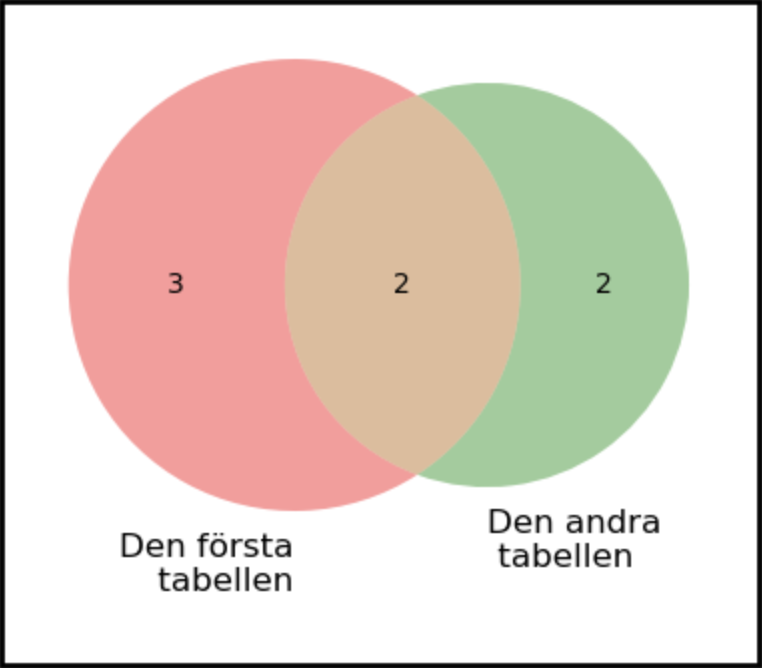
\includegraphics[width=120pt]{img_venn_diagram.png}};
\end{tikzpicture}
\if(x)
\begin{lstlisting}
!pip install matplotlib_venn
import matplotlib.pyplot as plt
from matplotlib_venn import venn2
# Example data
set1 = {'a', 'b', 'c', 'd', 'e'}
set2 = {'d', 'e', 'f', 'g'}
# Set up Venn labels and colors
venn_labels = {'100': set1 - set2, '050': set2 - set1, '140': set1.intersection(set2)}
venn_colors = {'100': 'red', '050': 'green', '140': 'blue'}
# Set figure size
plt.figure(figsize=(6, 6))
# Create a Venn diagram
venn2([set1, set2], set_labels=('Den forsta tabellen', 'Den andra tabellen'))
# Display the rectangle
plt.gca().add_patch(plt.Rectangle((-0.8, -0.8), 1.6, 1.4, fill=None, edgecolor='black', 
								   	     linewidth=2))
# Fine-tune the position of the labels
plt.text(-0.35, -0.9, 'Venn Diagram', ha='left', va='top')
plt.text(0.35, -0.9, '', ha='right', va='top', fontsize=12)
# Fine-tune the position of the figure
plt.subplots_adjust(top=0.9)
# Set equal aspect ratio
plt.axis('equal')
# Set plot limits
plt.xlim(-1, 1)
plt.ylim(-1, 1)
# Display the plot
plt.show()
\end{lstlisting}
\fi
\subsection{Indexering}

Indexering är att skapa en metod att söka och hitta en viss rad i en tabell utan att nödvändigtvis behöva iterera igenom varenda rad i den tabellen.



\subsection{Vy}

En vy är samma sak som en tabell och kan användas och hanteras på samma sätt. Det finns dock en väsentlig skillnaden; att en vy skapas i ramminnet och är tillgängligt att använda så länge databasen är aktiv och servern/ datorn är påslagen.



\subsection{Lagrad procedur}

Lagrad procedur, som namnet föreslår, är en samling av SQL-kommandon som redan har kompilerats och är redo för körning. Detta för att spara tid och minne, undvika redundans i koden och att ge möjligheten att tillhandahålla information till "extern" användare utan att denne ska ha direkt tillgång till databasen och källkoden.



\section{I praktiken}


\subsection{Bakgrund}

Databasen AdventureWork2022 är en fiktiv databas för att uppvisa Microsoft's möjligheter att hantera databaser i allmänhet. Den består av 5 scheman personal, kunder, tillverkning, försäljning, och återförsäljare, vilka i sig innehåller flera tabeller var. Originalen innehåller också redan flera vyer, vilket gör hopslagning (join) av tabellerna ännu enklare.

Det finns data om 296 anställda varav 290 jobbar kvar, 13 jobbkandidater, 181 försäljningsregioner, 1764 produkter, 6 cykelmodeller, 104 försäljningsställe med 156 kontaktpersoner, 19972 kunder och 17 säljare.

\subsubsection{Installation av programvara och import av bibliotek och moduler}

Förutom installation av \textbf{sqlalchemy} behövde vi importera \textbf{matplotlib.pyplot}, \emph{venn2} från \textbf{matplotlib\_venn}, \textbf{pandas}, \emph{LabelEncoder} from \textbf{sklearn.preprocessing}, \emph{datetime} från \textbf{datetime}, \textbf{seaborn}, \textbf{numpy}, \emph{stats} från \textbf{scipy}, samt \emph{sm} från \textbf{statsmodels.api}.

\subsubsection{Databas, uppkoppling och åtkomst}

Detta har redan diskuterats och behöver inte redovisas. Dock är det bra att påpeka att till vår \emph{engine} har vi använt parametervärdena 'mssql', 'DESKTOP-PJ0B80O', 'AdventureWorks2022', och integrated\_security=True.

\subsubsection{Förberedelse av scheman och tabeller}
 
 Detta är också redan diskuterat och behöver inte tas upp här.

\subsubsection{Databas förfrågan (Queries)}

Vi försöker först med att ta en snabb titt på alla tabeller i databasen (Cell ........).
\if(x)
\begin{lstlisting}
...
    for table in inspector.get_table_names(schema=sch):
        if sch != 'dbo':
            # Get the names of all the tables in each schema and
            # generate a string with all the queries
            col_names = ', '.join(col['name'] for col in 
            			      inspector.get_columns(table_name=table, schema=sch))
            full_table_name = f"{sch}_{table}"
            query = f"SELECT {col_names} FROM {sch}.{table}"
            ...
\end{lstlisting}
\fi
Resultatet blir en beskrivning av alla tabeller i databasen, vad vi har använt för \emph{Query}, de första fem raderna i tabellen och lite statistik över just den tabellen (Cell .........).
\if(x)
\begin{lstlisting}
QUERY
------
 SELECT DepartmentID, Name, GroupName, ModifiedDate FROM HumanResources.Department 
*************************************************************************
Schema: HumanResources
Table: Department

   DepartmentID         Name                 GroupName ModifiedDate
0             1  Engineering  Research and Development   2008-04-30
1             2  Tool Design  Research and Development   2008-04-30
2             3        Sales       Sales and Marketing   2008-04-30
3             4    Marketing       Sales and Marketing   2008-04-30
4             5   Purchasing      Inventory Management   2008-04-30
*************************************************************************
       DepartmentID         ModifiedDate
count     16.000000                   16
mean       8.500000  2008-04-30 00:00:00
min        1.000000  2008-04-30 00:00:00	75%       12.250000  2008-04-30 00:00:00
25%        4.750000  2008-04-30 00:00:00	max       16.000000  2008-04-30 00:00:00
50%        8.500000  2008-04-30 00:00:00	std        4.760952                  NaN
\end{lstlisting}
\fi

Vi noterar att schemas \emph{Person} och \emph{Sales} innehåller mycket information som är relaterade till företagets kunder. Detta väljer vi som ämne för vår analys och framställer samma tabeller ännu en gång för att lättare undersöka sambanden mellan tabeller som innehåller all information om kunderna. Koden skiljer sig inte annat än att vi bara väljer de tabeller som tillhör schemas Persona och Sales (Cell .......).
\if(x)
\begin{lstlisting}
...
    if sch == 'Person' or sch == 'Sales':
	    ...
\end{lstlisting}
\fi

Sedan att vi får en hel del tabeller som egentligen inte kommer till någon användning är något vi kan försumma när det kommer till automatisk utvinning of information, trots att det minskar överskådligheten. Detta eftersom vi ritar grafer för alla kolumner i alla tabeller, istället för att välja ut ''rätt'' kolumn, vilket skulle kräva mer analytisk kodskrivning genom t ex regex-uttryck (Cell ......... refer to figures).
\if(x)
\begin{figure}[h]
    \centering
    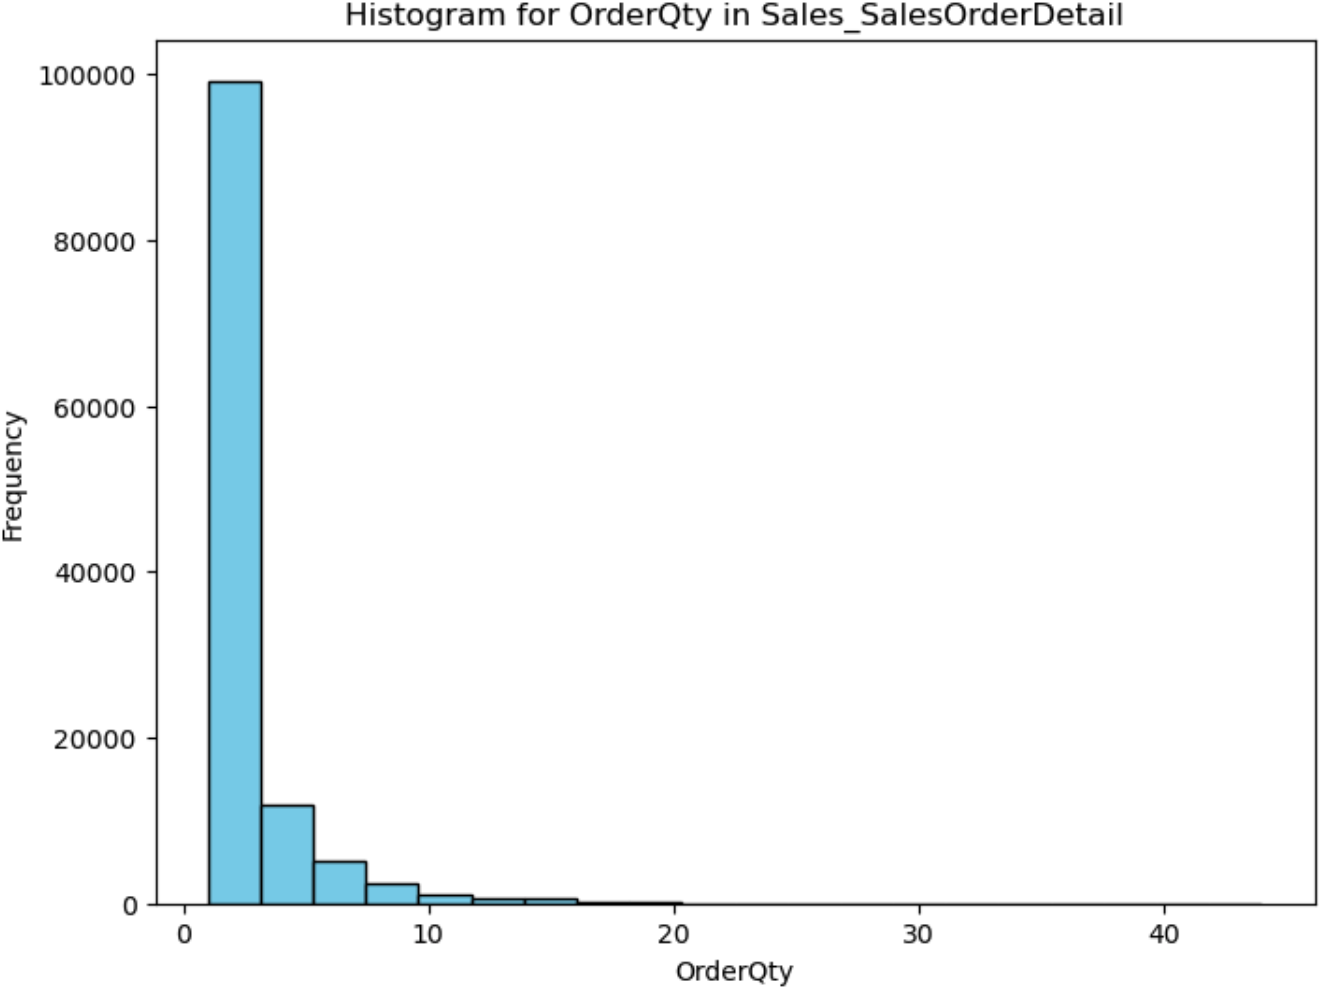
\includegraphics[width=0.7\textwidth]{img_order_quantity.png}
    \caption{Order Quantity.}
\end{figure}

\begin{tikzpicture}[remember picture,overlay]
    \node[anchor=north west, inner sep=0pt] at ([xshift=5pt, yshift=-300pt] current page.north west) {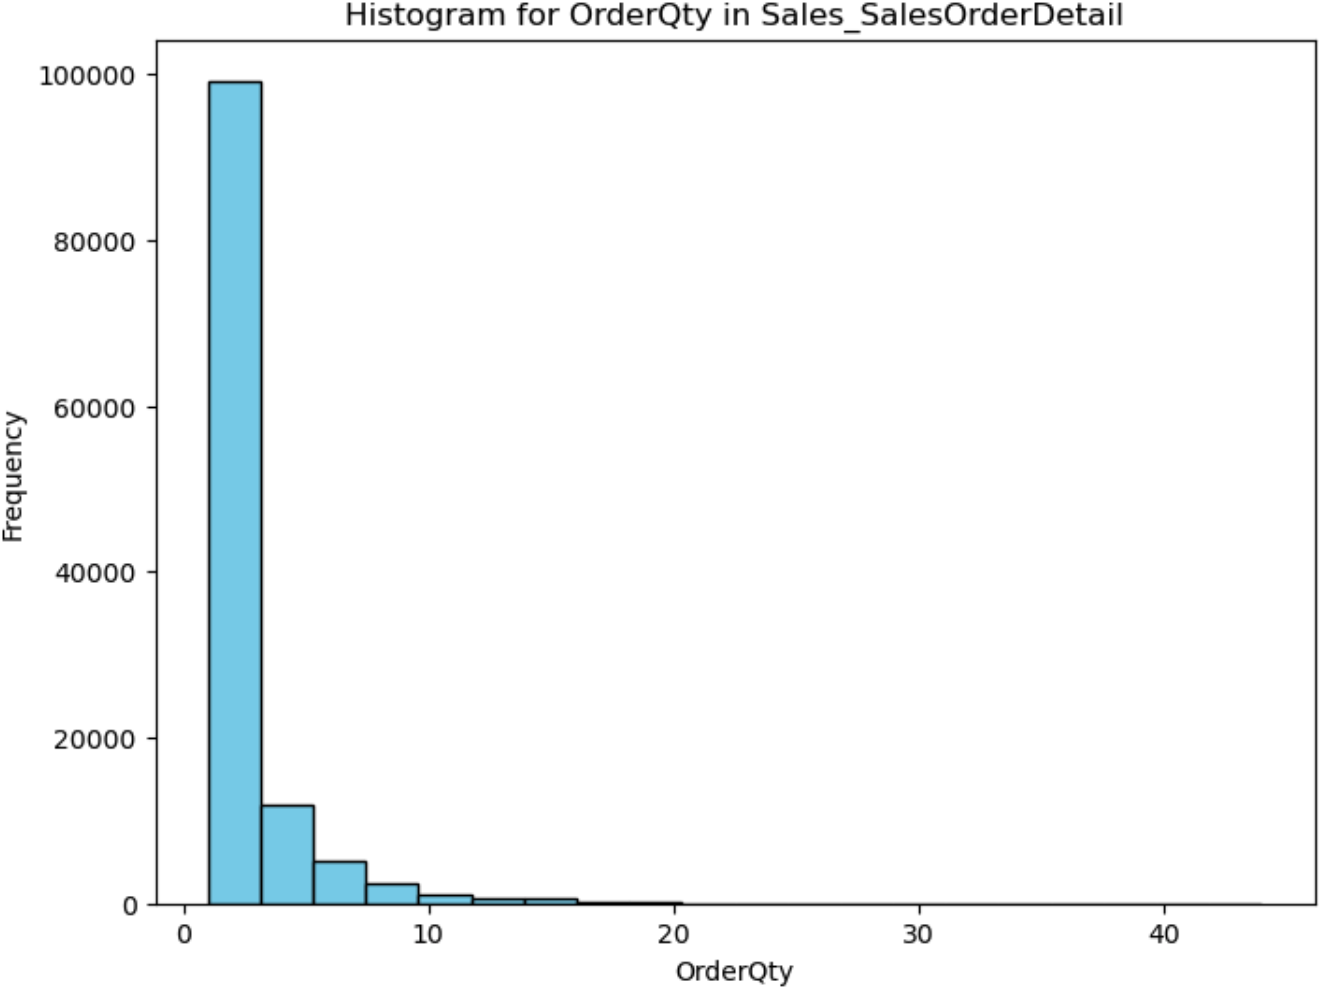
\includegraphics[width=240pt]{img_order_quantity.png}};
\end{tikzpicture}
\fi

Det var först här som vi noterade att det finns många egenskaper hos kunderna som skulle kunna undersökas närmare för att se ett mönster. Vi tittar också på views som redan finns presenterade i den originella databasen och speciellt där kunderna är uppradade. Den största skillnaden mot tidigare koder är att vi istället använder \emph{inspector.get\_view\_names} (Cell ........)
\if(x)
\begin{lstlisting}
...
    for sch in schemas:
        for view in inspector.get_view_names(schema=sch):
            ...
\end{lstlisting}
\fi

Vi bestämmer oss således för att jämföra köpvanan hos kvinnor och män och undersöka om vi kan hitta olika mönster i hur män och kvinnor investerar i sin hälsa/ ekonomi, alternativt för en miljövänligare transportmedel. Från de senaste utskrifterna kan vi konstatera att för en rättvis och noggrann jämförelse mellan könen behöver vi tabeller med många kunder i. Därför väljer vi \emph{vIndividualCustomer} och \emph{vPersonDemographics} från schema \emph{Person}. Vi gör en \emph{JOIN} mellan de två tabellerna och får (Cell ............)
\if(x)
\begin{lstlisting}
# SQL query for joining the two tables
joint_table = f'''
                SELECT *
                FROM Sales.vPersonDemographics AS VPD
                JOIN Sales.vIndividualCustomer AS VIC
                ON VIC.BusinessEntityID = VPD.BusinessEntityID;
            '''
# Save the result in a data frame for further investigation
joint_df = pd.read_sql(sql=joint_table, con=connection)
print(joint_df.head(5))
\end{lstlisting}
\fi

Vi gör en klassificering av data i kolumnen för årsinkomst och får
\if(x)
\begin{lstlisting}
# Count the number of incomes on each income level
income_counts = joint_df['YearlyIncome'].value_counts()
print(income_counts)
\end{lstlisting}
\fi

\begin{figure}[h]
    \centering
    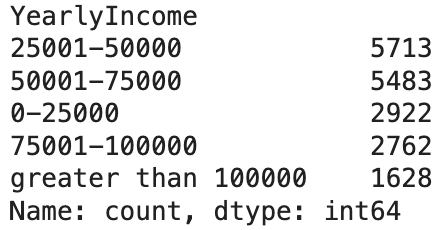
\includegraphics[width=0.25\textwidth]{img_yearly_income.png}
%    \caption{Yearly Income}
\end{figure}

\if(x)
\begin{tikzpicture}[remember picture,overlay]
    \node[anchor=north west, inner sep=0pt] at ([xshift=400pt, yshift=-9.0in] current page.north west) {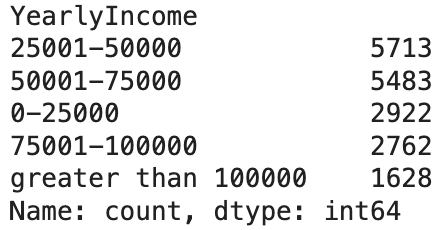
\includegraphics[width=120pt]{img_yearly_income.png}};
\end{tikzpicture}
\fi



För att kunna använda denna kolumn i våra statistiska beräkningar ersätter vi varje intervall med dess max-gräns, dvs:
\begin{itemize}[topsep=10pt, partopsep=0pt, itemsep=0.2em, parsep=0pt]
	\item[] 0-25000 with \textbf{25,000}
	\item[] 25001-50000 with \textbf{50,000}
	\item[] 50001-75000 with \textbf{75,000}
	\item[] 75001-100000 with \textbf{100,000}
	\item[] greater than 100000 with \textbf{500,000}
\end{itemize}
för att göra talen i kolumnerna konvertibla till heltal inför nästa steg som är att skapa en korrelationsmatris. Vi kommer inte att använda själva talen i våra beräkningar så det finns ingen risk att våra beräkningar genererar felaktiga resultat. Med andra ord använder vi årsinkomsten endast som en ordinal, kategorisk variabel. (Cell pattern = r'-(\d+)| (\d+)')

\subsubsection{Övergång från kategorisk data till ordinal data}

Bortsett från födelsedatum för kunderna är varken omvandlingen eller kategoriseringen lika komplicerade att utföra för de andra kolumnerna. Här använder vi \emph{LabelEncoder}  (Cell 322 och 323) till att beräkna företagskunders respektive ålder. För de andra kolumnerna (Cell 326 till 331) är det som sagt inte like dramatiskt utan alla följer samma mönster.

\section{Analys och slutsatser}

\subsection{Ett första försök: hitta samband mellan Total Purchase YTD och andra faktorer}

Innan vi går vidare med att jämföra könen, gör vi en analys för att se om det eventuellt finns något samband mellan det belopp man spenderat under det nuvarande året och något av de relevanta egenskaperna hos företagets kunder. Vi kan använda de nya kolumnerna till att beräkna korrelationen mellan alla dessa variabler, med hopp om att hitta variabler som är mer korrelerade med andra, speciellt de som är kopplade till kundernas kön.

Från tabellen kan vi endast utläsa vilka par av variabler som är mer korrelerade än andra, nämligen: Agex-Loyaltyx (0.9; detta är framför allt pga vår egen definition of Loyalty), Agex-TotalChildren (0.5), NumberChildren-TotalChildren (0.5), YearlyIncome-NumberCarsOwned (0.5), TotalChildren-Loyaltyx (-0.5), Inga av dessa är relevanta för vår studie och därför överger vi den undersökningen och söker lycka någon annanstans.

Den enda finansiellt relevanta slutsats vi kan dra är att lojalitet är "mot-korrelerad" mot antal barn som i sin tur är korrelerad med ålder. Detta betyder att de äldre tenderar att visa mindre lojalitet, vilket kan förstås i och med att de äldre har fler barn och både har mindre tid att handla och mindre pengar att spendera på egna intressen.

I nästa steg tittar vi på inkomster och försöker hitta ett samband mellan könen och hur mycket de tjänar och spenderar. Eftersom den figuren inte tillför så mycket information lägger vi den inte till här. (Cell ........)
% The figure is on the top of the next page
\if(x)
\begin{figure}[h]
    \centering
    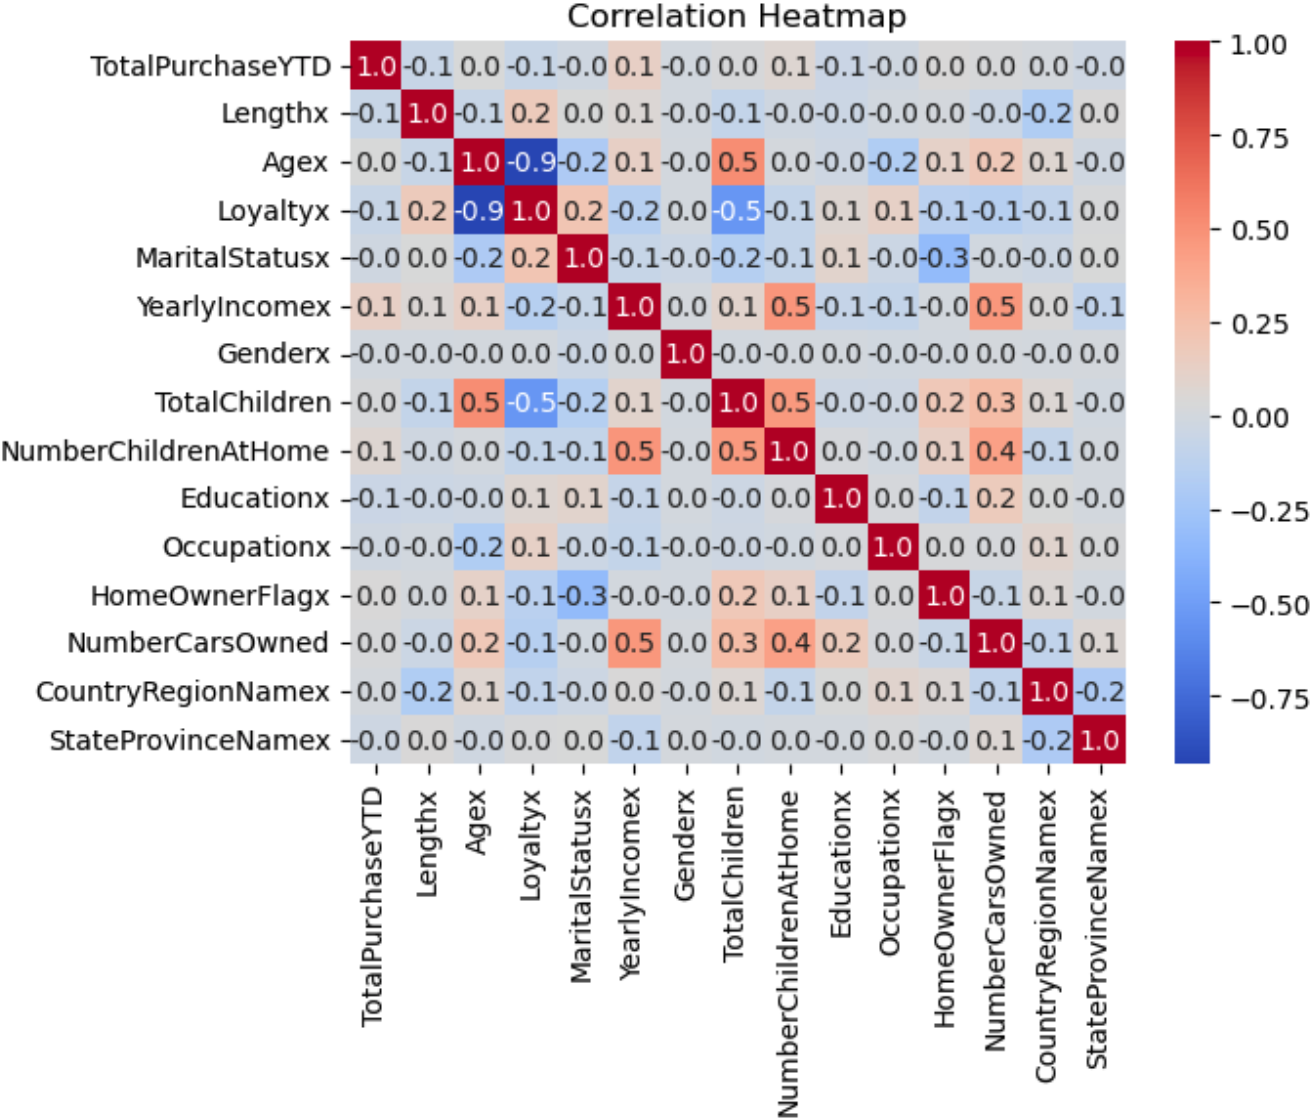
\includegraphics[width=0.6\textwidth]{img_correlation_heatmap.png}
    \caption{Correlation HeatMap}
\end{figure}
\fi







\subsection{Första 0-hypotensen: det finns skillnad i inkomst och köpvana hos de ''mest entusiastiska'' männen och kvinnorna}

Cell 334 visar kod som tar reda på exakt hur många olika inkomster som finns. Eftersom dessa uppgår till 3994 stycken olika värden väljer vi att dela dem i inkomstnivåer; i 30 nivåklasser (bins=30); som det framgår från Cell 335. I histogrammen på nästa sida ser vi en viss skiftning i kvinnornas totala köp i det föreliggande året jämfört med männens. Även i vår Boxplot ser vi denna skiftning, med extremvärden som ligger längre bort från "boxen" jämfört med schemat för männen. Därför finns det en chans att vi åtminstone kan hitta en 95 procentig signifikant skillnad.
\begin{figure}[h]
    \centering
    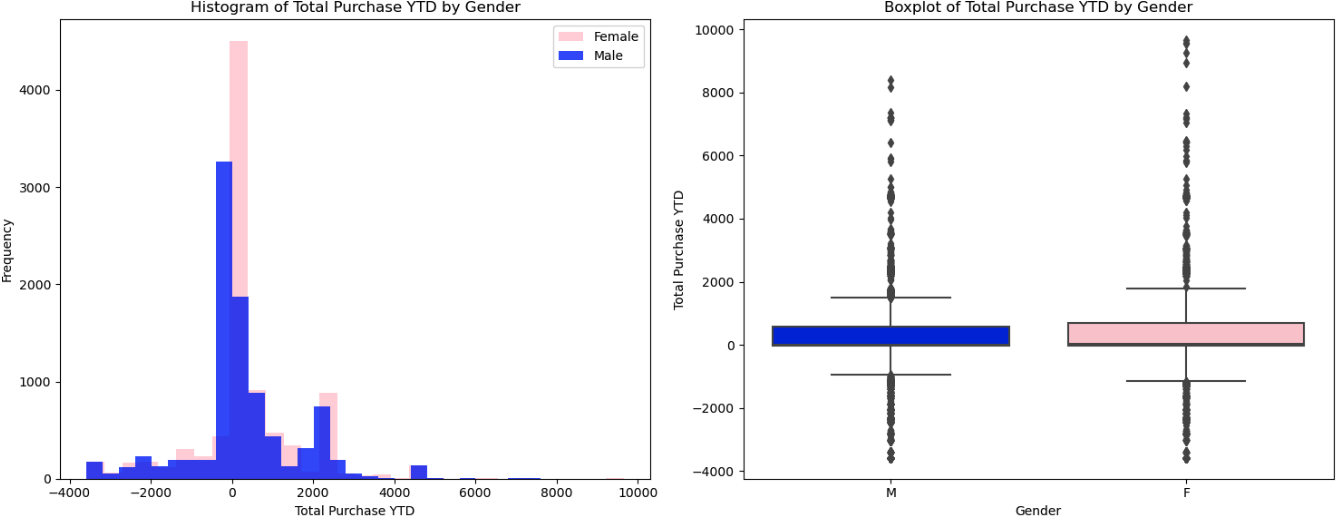
\includegraphics[width=0.98\textwidth]{img_boxplot.png}
%    \caption{Boxplot.}
\end{figure}
Detta betyder att det inte finns någon signifikant skillnad i generella drag mellan hur mycket män och kvinnor spenderar på köp av cykel och tillbehör.
\begin{figure}[h]
    \centering
    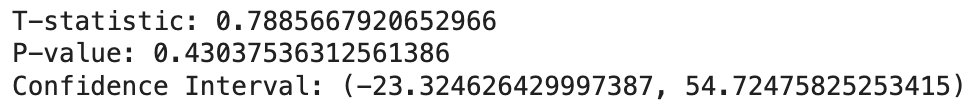
\includegraphics[width=0.6\textwidth]{img_gender_total_purchase_ytd.png}
    \caption{Gender TotalPurchaseYTD.}
\end{figure}








\subsection{Andra 0-hypotensen: det finns en signifikant skillnad mellan könen i den högre ''spenderarklassen''}

Om vi tittar på spridningsdiagrammet för hela populationen, märker vi att de högsta beloppen spenderas av de som är mellan 40 och 55 år gamla.
\begin{figure}[h]
    \centering
    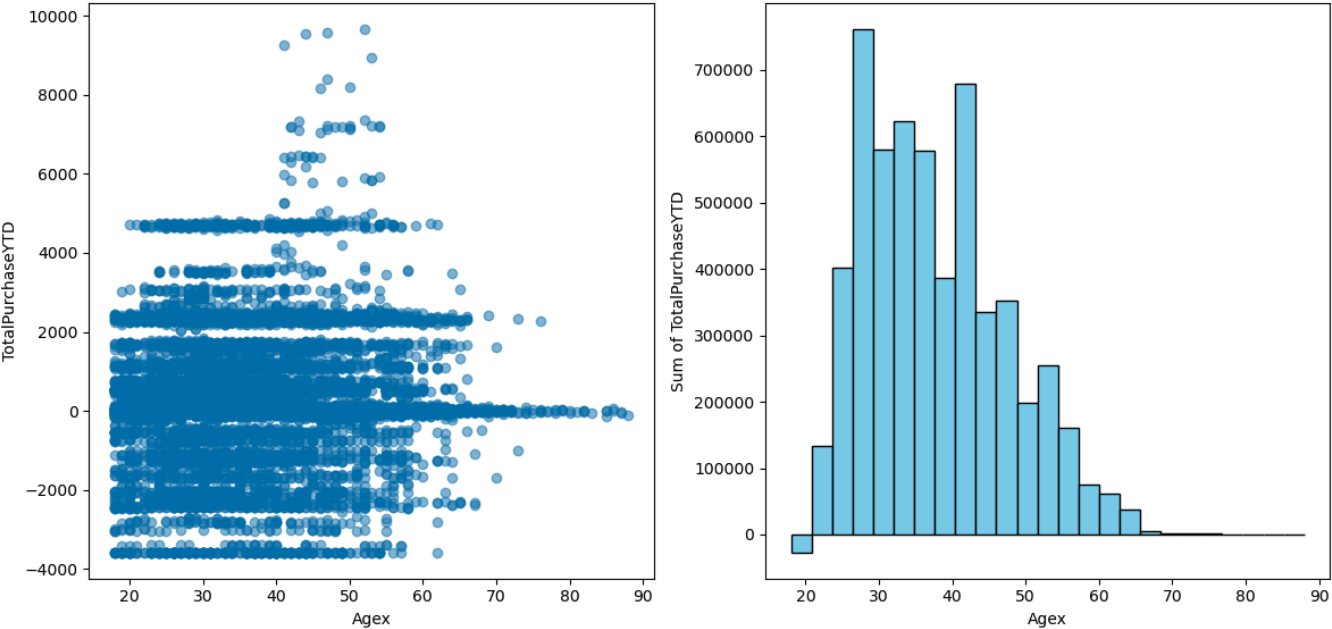
\includegraphics[width=\textwidth]{img_total_purchase_ytd_agex.png}
    \caption{TotalPurchaseYTD agex}
\end{figure}
Så vi separerar den gruppen som spenderar mer än 5000 dollar per år och tittar på skillnaden mellan män och kvinnor inom den gruppen av kunder.
\begin{figure}[h]
    \centering
    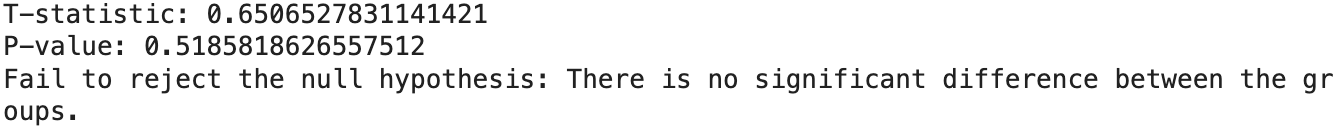
\includegraphics[width=0.8\textwidth]{img_spenderarklassen.png}
%    \caption{Spenderarklassen.}
\end{figure}
Vi finner återigen ingen signifikant skillnad mellan dessa värden.








\subsection{Tredje 0-hypotensen: det finns en signifikant skillnad i köpvana mellan kvinnor och män i de olika inkomstklasserna}

Efter att inte ha lyckats med att hitta någon skillnad mellan de från båda könen som spenderar mest på köp av cyklar och tillbehör, gör vi ett försök med att se om det förekommer någon signifikant skillnad i hur mycket män och kvinnor i varje inkomstklass.
\begin{figure}[h]
    \centering
    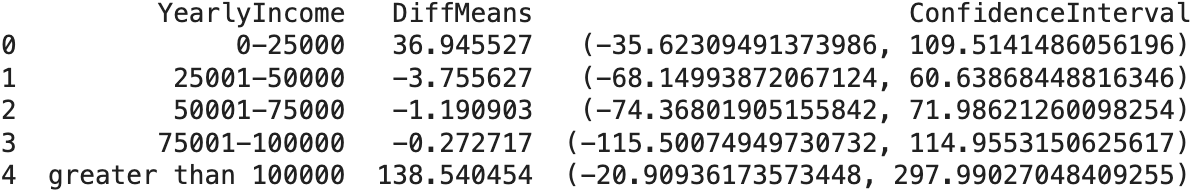
\includegraphics[width=0.7\textwidth]{img_income_classes.png}
    \caption{Income Classes.}
\end{figure}

spenderar på sin hobby iår.
\begin{figure}[h]
    \centering
    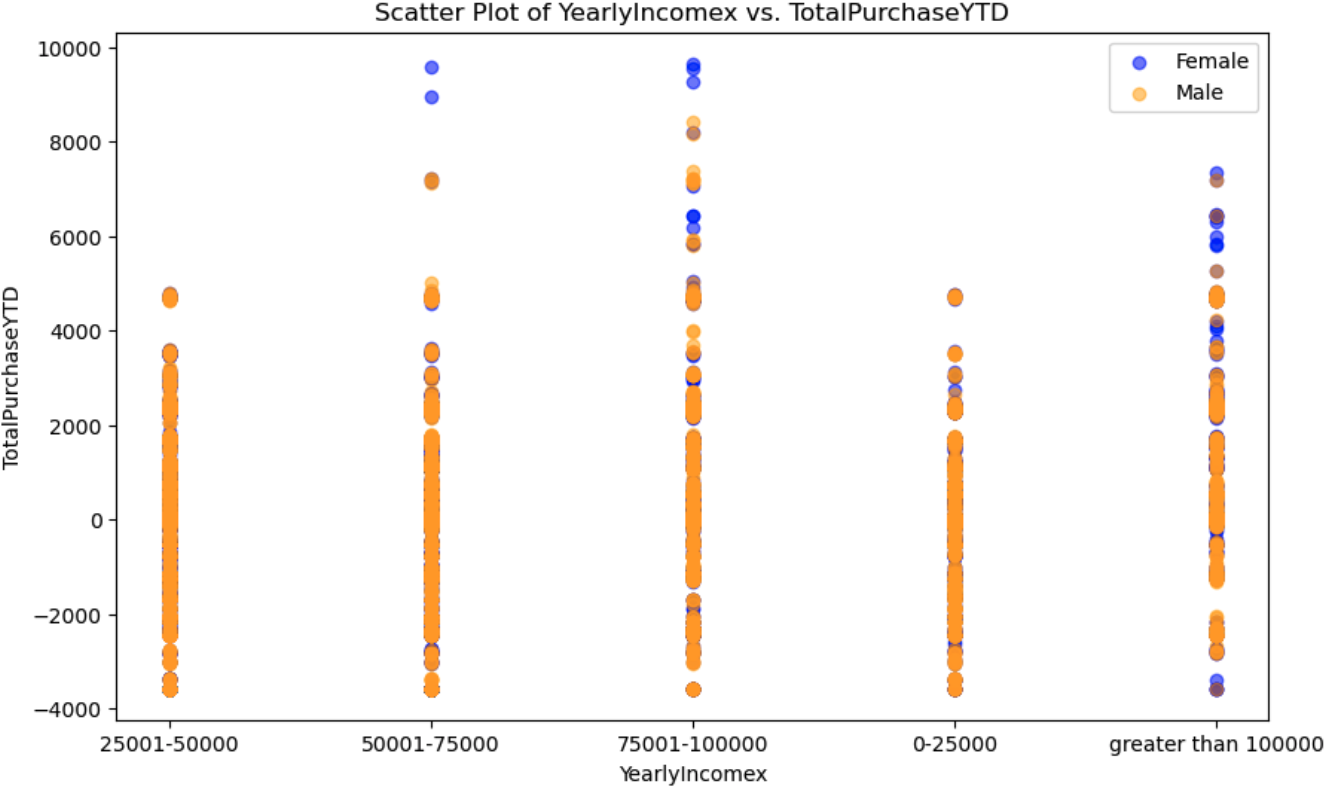
\includegraphics[width=\textwidth]{img_shopping_habbit_for_income_classes.png}
    \caption{Shopping habbit for Income Classes.}
\end{figure}

Även här hittar vi alltså ingen signifikant skillnad mellan män och kvinnors köpvana, när det kommer till cykel och tillbehör.

\section{Conclusion}

Genom att titta på fyra olika hypoteser har 



\section{Framtida undersökningar}

Det finns fortfarande saker att undersöka, exempelvis genom att dela beloppet man spenderat under året med ens årliga inkomst kan man också hitta ny information som kan vara en skiljepunkt mellan män och kvinnor, även om informationen vi hittills bearbetat fram inte tyder på det.

Generellt sett, skulle man också kunna använda multipel regression för att eventuellt kunna hitta samband mellan flera variabler samtidigt. Detta ingår dock varken i statistik- eller den föreliggande kursen och har därför inte beaktats.

\end{document}